\chapter*{If you have never used \emph{Mathematica} \ldots }
\label{chap:Prelim}

This pamphlet assumes you have done at least a little programming before, possibly in C, C++, FORTRAN, Visual Basic, or some other language. If not, \emph{that is completely fine}. We will walk you through some simple programming concepts here so that you can get your feet wet, and then you will be ready to take on chapter 1.

If you have done some programming before, but have never used \emph{Mathematica}, it will still benefit you to spend some time with this section, because it will walk you through some tricks to make using \emph{Mathematica} more pleasant.

\section{Notebooks and Cells}

When you start \emph{Mathematica} for the first time, it will create a new \emph{notebook} for you. A notebook is just a type of document, like a Microsoft Word document, but it is specially designed to make \emph{Mathematica} programming easier.\footnote{Note that for most programming languages, you type your code in a \emph{plain text} document, or one that has no special formatting in it. This is not the case in \emph{Mathematica}; if you open a notebook in Vim or Notepad, you will see that your code is surrounded by lots of formatting directives that you probably don't want to type by hand!} Notebooks are broken into cells, which you can think of like paragraphs. Each cell can have code in it, and they can be evaluated\footnote{To ``evaluate'' some code simply means to run it.} independently.

You can create new cells by clicking in a blank region of the docoument. You will see the cursor displayed sideways, and that is \emph{Mathematica}'s way of telling you that the cursor is in between cells or that it is not inside a cell. As soon as you start typing anything, a new cell will be created, your cursor will hop inside, and anything you type will be displayed there.

Cells can have different ``Styles'' depending on what you want to use them for. By default, when a new cell is created it will be an ``Input'' cell, which means you can type code in it and evaluate it. By right-clicking on the vertical bar on the right side of a cell, you can bring up a menu that will allow you to change the style of the cell. Changing your cell style to ``Title'', ``Section'', ``Subsection'', etc. as appropriate can help you organize your work and will make your presentations look more professional.

When you type some code in a cell, you can evaluate it by pressing ``Shift+Enter''\footnote{In case you are not familiar with this convention, it means to hold the ``Shift'' key and then press the ``Enter'' button}

\section{Fancy Typing and the Palette}

When you start \emph{Mathematica}, it should load a set of buttons in a thin vertical window to the right of your notebook. If it does not, you can access this palette by going to ``Window'' $\rightarrow$ ``Palettes'' $\rightarrow$ ``Basic Math Input'' in the menu bar. The palette gives you ways to make your code look more mathematical. For example, there are buttons for writing integrals, summations, exponents, matrics, greek letters, etc.\footnote{Indeed, many of the basic features of \LaTeX are available in \emph{Mathematica} to help you typeset mathematical expressions, but you will still need the full power of \LaTeX in order to prepare your research for publication}. If you press any of these buttons, it will insert the necessary symbols into the current cell and you will see several small boxes in the positions where one would expect symbols. Pressing ``Tab'' will allow you to move between these boxes, and type any valid \emph{Mathematica} expression in them.

\subsection{Subscripts, Exponents, and Fractions}

There are also keyboard shortcuts for many of the symbols in the palette. For example, to type a fraction, you can press ``Ctrl+/'' and your cursor will automatically be placed in the numerator. To type the fraction $\frac{2}{3}$ in \emph{Mathematica}, you simply need to press ``Ctrl+/'' and then ``2'', ``Tab'' (which moves you to the denominator), and then ``3''.

Likewise, to type $x^3$, you simply type ``x'' and then ``Ctrl+6'' and then \emph{Mathematica} will give you a black box above and to the right of the ``x'' character and move your cursor there. Then type ``3'', and you will have $x^3$.

You can of course combine elements in expression boxes. For example, to write $x^{\frac{2}{3}}$, you can type ``x'' and then ``Ctrl+6'' to get an expression box in the exponent position, then type ``Ctrl+/'' to turn that box into a fraction, then hit ``2'', ``Tab'', and then ``3''.

\subsection{$\pi$, $\theta$, and $alpha$}

Using the ``Esc'' button, you can generate these symbols. ``Esc+pi+Esc'' will get you the $\pi$ symbol. You can look at Table \ref{tab:GreekLettersTable} to see a longer list of symbols. These symbols are also available in the ``Basic Math Input'' palette.

\begin{table}
	   \centering
	   \begin{tabular}{ll}
			 Symbol & \emph{Mathematica} code \\
			 $\pi$ & ``Esc'' pi ``Esc'' \\
			 $\alpha$ & ``Esc'' alpha ``Esc'' \\
			 $\beta$ & ``Esc'' beta ``Esc'' \\
			 $\theta$ & ``Esc'' theta ``Esc'' \\
			 $\phi$ & ``Esc'' phi ``Esc'' \\
			 $\eta$ & ``Esc'' eta ``Esc'' \\
			 $\chi$ & ``Esc'' chi ``Esc'' \\
	   \end{tabular}
	   \caption{A table of greek letters}
	   \label{tab:GreekLettersTable}
\end{table}

\subsection{Sums, Integrals, and Derivatives}

These are best accessed by using the corresponding buttons in the ``Basic Math Input'' palette. For example, clicking on the large capital Sigma will give you a summation sign with two input boxes below it and one above. You can type expressions in these boxes and press ``Tab'' to go to the next. You can also construct integrals and derivatives in this fashion. Here are some things to try:

\begin{enumerate}
	   \item Find the sum $\sum_{n=1}^{10} 2^n$
	   \item Make \emph{Mathematica} show you that $\int_0^{\pi} \sin(x) dx = 1$
	   \item Find the derivative of $\sin(x)$
\end{enumerate}

\section{Functions}
\emph{Mathematica} has tons of built-in functions. It has trig functions like \texttt{Sin} and \texttt{Cos}. It also has functions for plotting graphs and generating lists or tables of data (see ``\nameref{chap:Plotting}'' and ``\nameref{chap:ListsMap}''). In addition, you can create your own functions, but that will be discussed in Chapter \ref{chap:Functions} \nameref{chap:Functions}. For now, it is important to go over a few basics about how functions work in \emph{Mathematica}.

For example, we know from trig that $\sin(\frac{\pi}{2}) = 1$. To see this for yourself in \emph{Mathematica}, type the following into a cell:

\begin{code}
	   Sin[pi/2]
\end{code}
and press ``Shift+Enter'' to evaluate the cell. Below, you will see an output cell generated containing the number 1. However, there are other functions in \emph{Mathematica} aside from normal math functions. For example, you can use the \texttt{Map} function to produce a list of sine values for a given set of domain points. 

To see what we are talking about more clearly, let's consider the set $(0, \frac{\pi}{2}, \pi, \frac{3\pi}{2}, 2\pi)$. We can calculate the corresponding range values very simply by applying \texttt{Sin} to these values via \texttt{Map}.

\begin{code}
	   Map[Sin, {0, pi/2, pi, 3pi/2, 2pi}]
\end{code}
and you will see that this produces the ranges values $(0, 1, 0, -1, 0)$.

\section{Variables}
\emph{Mathematica}'s variables are very simple. Variables can hold numbers, lists, matrices, functions, symbols, or graphs. For now, we will just look at how to store some numbers as variables and see how it affects a plot.

\begin{code}
	   Amplitude = 1;
	   UpperBound = 10;
	   Plot[Amplitude * Sin[x], {x, 0, UpperBound}]
\end{code}

\begin{figure}[t]
\centering
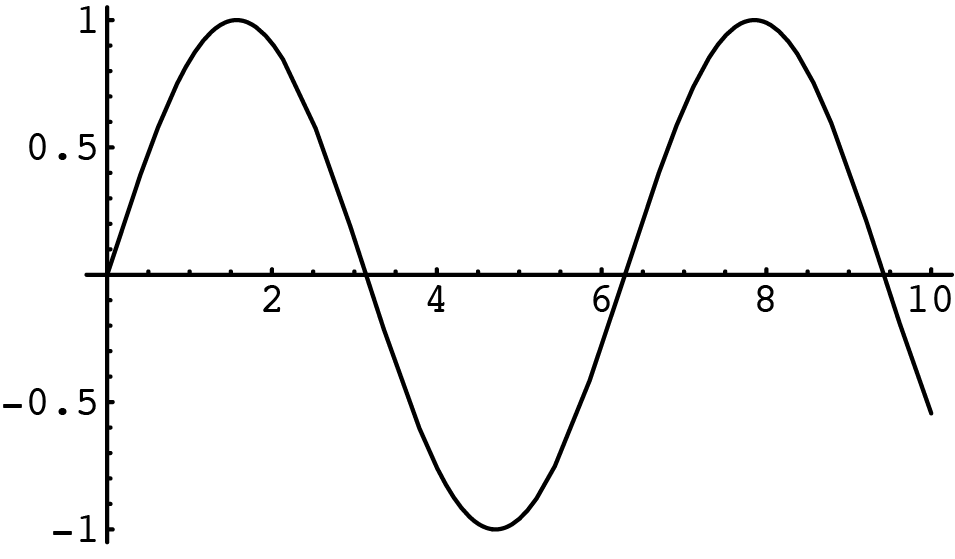
\includegraphics{figures/Preliminaries/SineWithAmplitudeAndUpperBound}
\caption{Output from the above Cell}
\label{fig:Preliminaries_SineWithAmplitudeAndUpperBound}
\end{figure}

When you execute this, you will see that $\sin(x)$ will be drawn on the interval $(0,10)$. Try doing the following by changing the values for \texttt{Amplitude} and \texttt{UpperBound}:


\begin{enumerate}
	   \item Plot $2\sin(x)$ on $(0,10)$
	   \item Plot $-\sin(x)$ on $(0,10)$
	   \item Plot $\pi\sin(x)$ on $(0, 2 \pi)$
\end{enumerate}
